\chapter{Setup}
\section{Protein structure}
All simulations were carried out with starting configurations adapted from previous work in the group (C36 forcefield: \textcite{pap003}, \martini{} forcefield: \textcite{sara}). These configurations contain only a FERM-kinase fragment without the FAT domain and its linker (only residues 35 to 686, PDB 2J0J \autocite{structFAK}).\\
As explained in \autoref{subsub:coarsegraining}, the secondary structure of proteins has to be stabilized in \martini{} using elastic networks. This was set up by \textcite{sara} to act only between backbone beads of the same domain which are within a cut-off radius of $1\,\si{\nano\metre}$. Therefore, the interface between FERM domain and kinase is not affected and the linker is still flexible. The force constant is 830 $\si{\kilo\joule\mole^{-1}\nano\meter^{-2}}$.
\section{Setup 1 - Free energy of basic patch}
\label{setup:setup1}
For this setup only a part of F2 (residues 107 to 219, referred as F2 lobe in the following) was used. The lobe contains the basic patch and has a net charge of -5. Therefore no additional ions were needed.\\
We placed the lobe as a \charmm{} structure above a single \pip{} embedded into a phosphatidylethanolamine (\pope{}) membrane (see \autoref{setup:setup2_pic}). After a short equilibration, the F2 lobe was pulled slowly away from the membrane using a distance pull between the COM of the lobe and the COM of \pip{}. From this simulation, we retrieved starting conformations for the umbrella window. The number of umbrella windows was chosen accordingly to the sampling (between 90 and 120 windows). Each window was shortly equilibrated and afterwards simulated for $6\,\si{\nano\second}$.  From the trajectories of the umbrella windows, the free energy profile was calculated using \gromacs{} WHAM implementation \autocite{gromacsWHAM}. The pulling and umbrella sampling was carried out five times to estimate the statistical error.\\
The starting configuration was transferred to a \martini{} structure (with both standard water model and PW) with the provided transformation tools \autocite{backwardpy}. Afterwards the elastic network was applied. Analogously to the simulation in \charmm{}, we retrieved starting configurations for the umbrella windows and simulated them for five independent copies. The simulation time for one umbrella window was increased to $10\,\si{\nano\second}$.\\
The presented results are based on a total simulation time of $3.88\,\si{\micro\second}$ for C36, $6.33\,\si{\micro\second}$ for \martini{}, $5.64\,\si{\micro\second}$ for \martini{} with PW. The temperature in the simulations was kept at $300\,\si{\kelvin}$. For all three force fields the default parameters were used.
% C36: 1=180, 4.2=135, 5=102, 5.2=102, 6=127, Mart: 1=134, 2=126, 3=130, 4=113, 5=130, MartPol: alle=113
%
%
%
\begin{figure}[t]
	\centering
	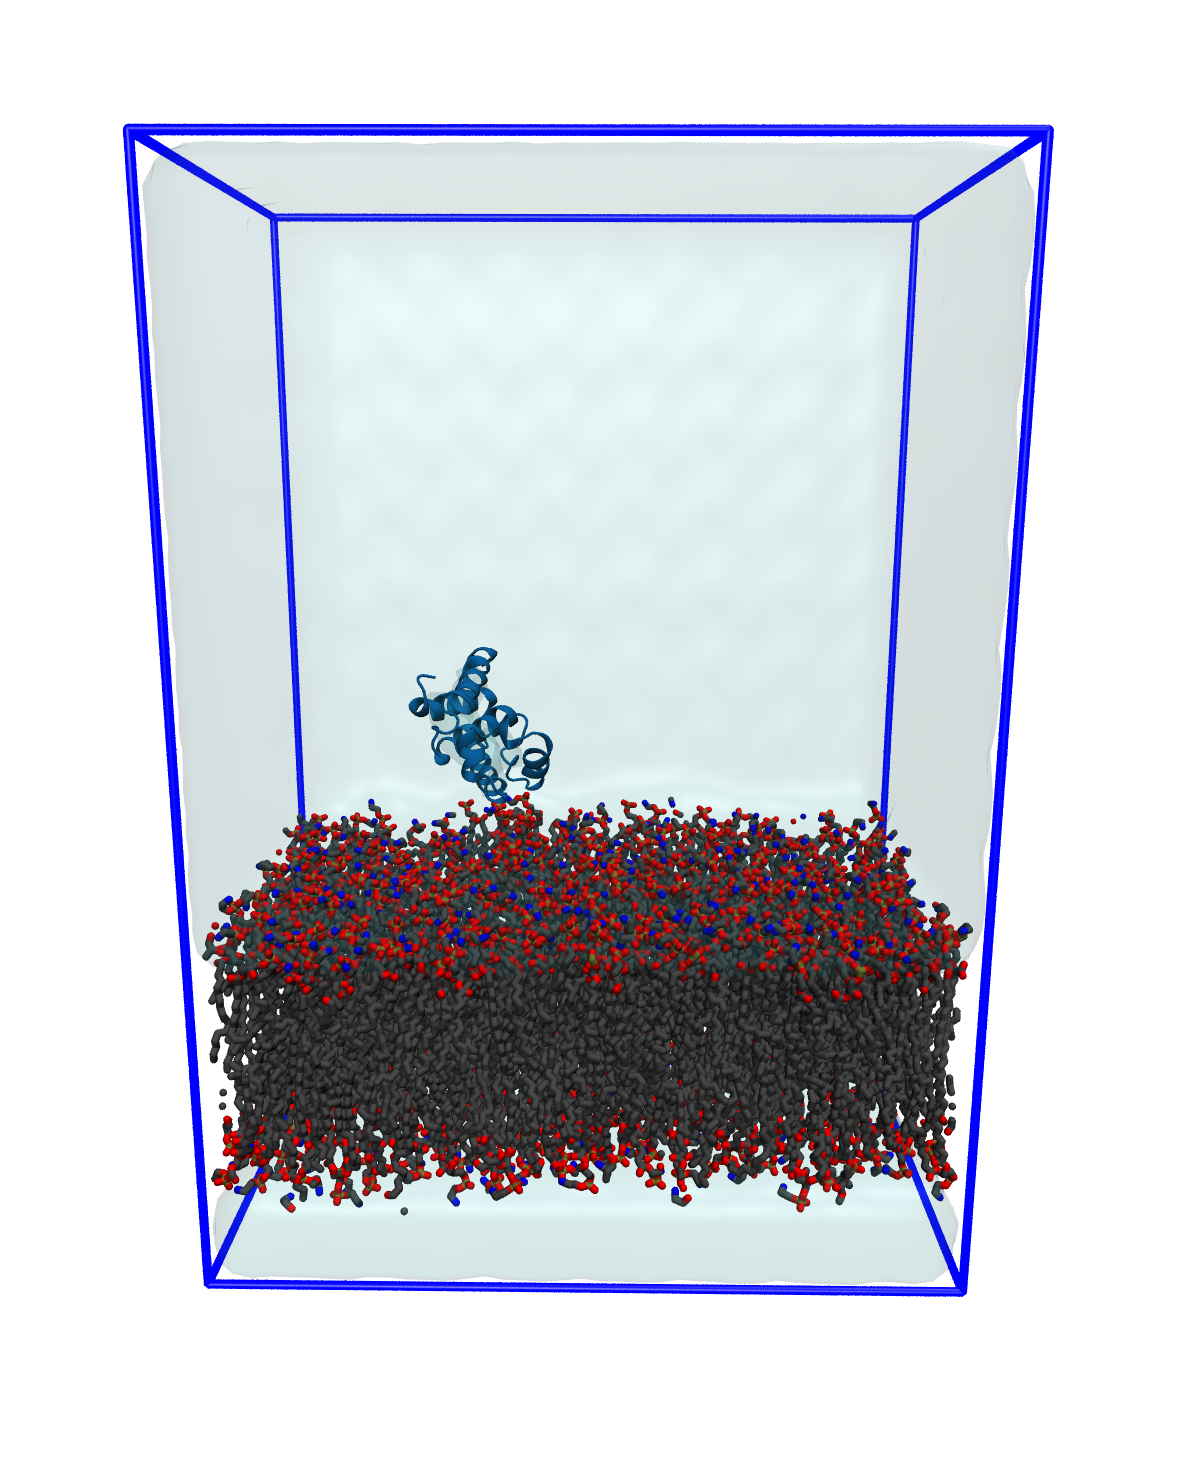
\includegraphics[height=5.5cm]{figures/setup/setup_umbrella}
	\nicecaption{Setup 1 - Free energy of basic patch}{The \charmm{} structure of the lobe (1936 atoms) above one \pip{} (143 atoms) embedded in a \pope{} membrane (509 lipids, ca. 63600 atoms). The box was filled up with ca. 63000 water molecules. The corresponding \martini{} structure contains 269 beads for the lobe, ca. 6100 beads for the membrane and ca. 16200 solvent beads/PW molecules. The box dimensions are $14.0\,\si{\nano\metre}$ x $9.0\,\si{\nano\metre}$ x $20.0\,\si{\nano\metre}$.}
	\label{setup:setup2_pic}
\end{figure}
%
%
%
\section{Setup 2 - FAK in solution}
\label{setup:setup2}
Setup 1 refers to a \martini{} simulation of a single FAK molecule in waterbox. NaCl ions were added to neutralize the charge (see \autoref{setup:setup1_pic}).\\
After a short equilibration the system was simulated for $20\,\si{\micro\second}$ at a temperature of $300\,\si{\kelvin}$. We used the default parameters of the \martini{} forcefield as input parameters.
%
%
%
\begin{figure}[hb]
	\centering
	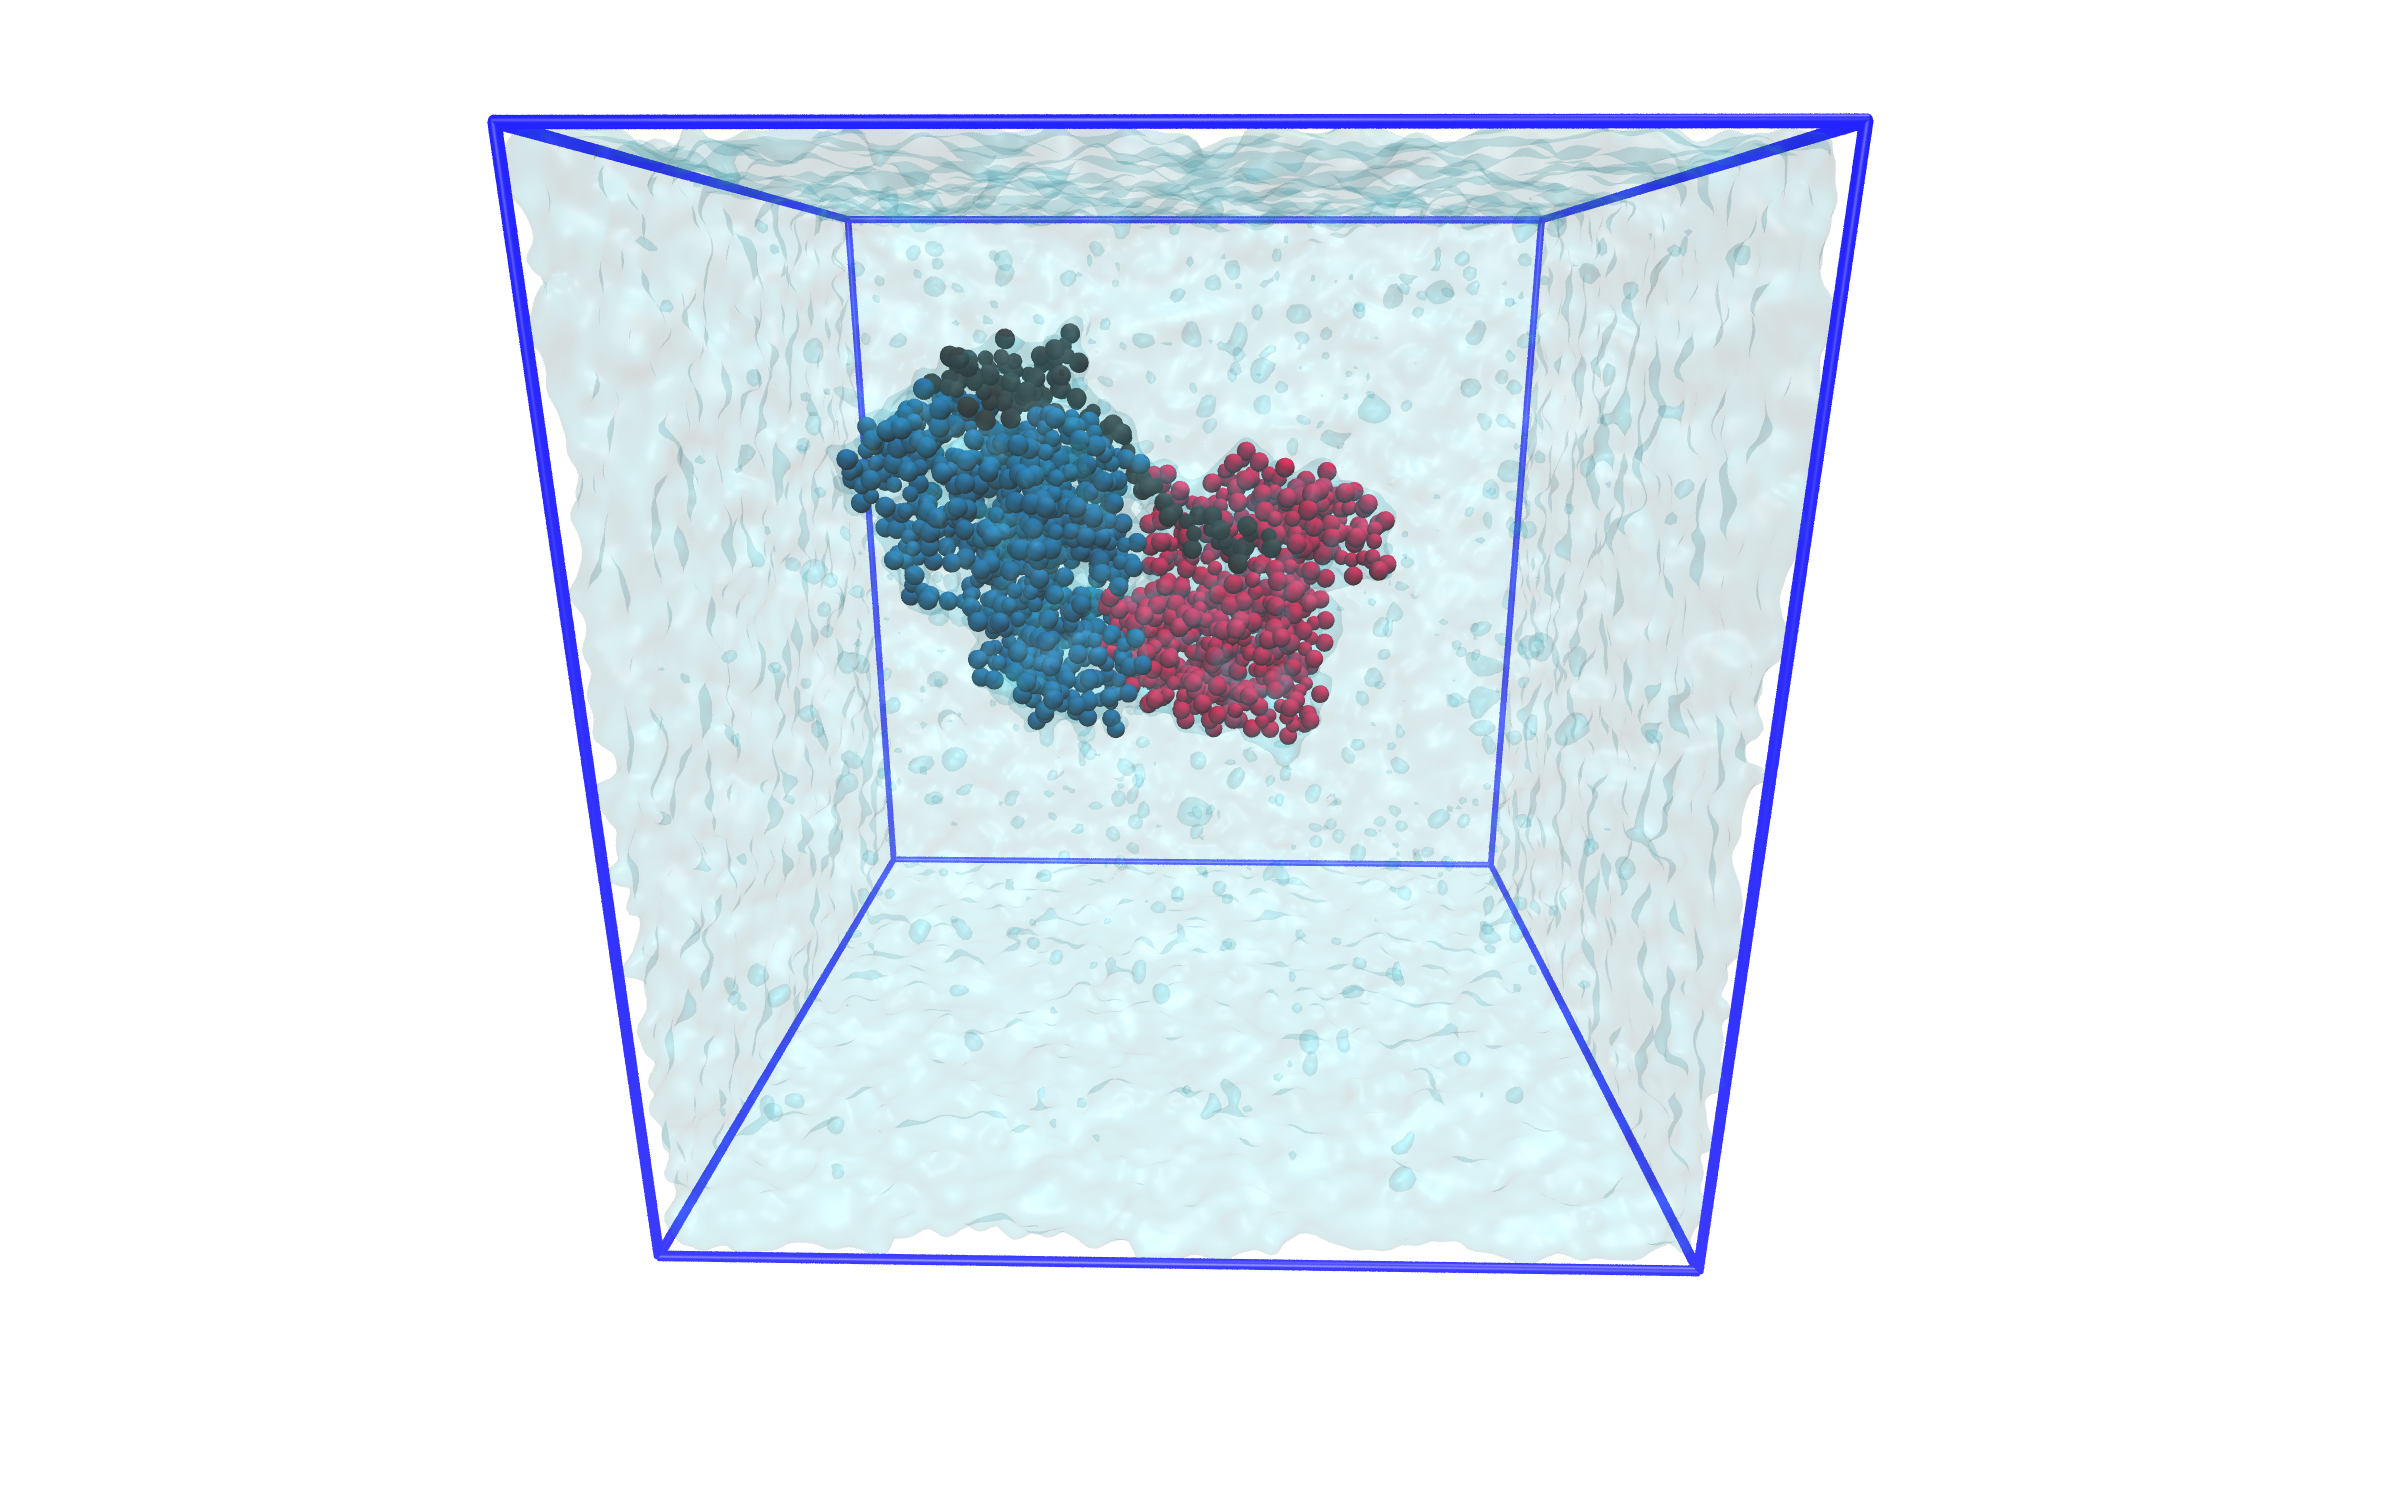
\includegraphics[height=5cm]{figures/setup/setup_free}
	\nicecaption{Setup 2 - FAK in solution}{The \martini{} structure of FAK (FERM blue, kinase red and linker black, 1486 beads) was put in a waterbox (ca. 50000 solvent beads) with ions (23 sodium beads and 20 chlorine beads). The box dimensions are $18.8\,\si{\nano\metre}$ x $18.8\,\si{\nano\metre}$ x $18.8\,\si{\nano\metre}$.}
	\label{setup:setup1_pic}
\end{figure}
%
%
%
\section{Stabilising force for FAK molecules}
\label{stabilising}
Unfortunately, previous work in the group revealed problems in the use of \martini{} regarding simulations of FAK, which are summarized in the following \autocite{sara}.\\
\textcite{sara} obtained in simulations of a single FAK molecule on a \pip{}-containing membrane rapid changes in the inclination of the protein with respect to the membrane. In the following, this inclination is characterized by the angle $\beta$ between the z-axis and the vector connecting F1 and F2, $\vec{d}_\text{F}$. $\beta$ is given as
\begin{equation}
\cos\left(\beta\right) = \frac{\vec{d}_{\text{F}, z}}{d_\text{F}},\quad d_\text{F} = \left|\vec{d}_\text{F}\right|.
\end{equation}
The distributions of $\beta$ for different simulations ($10\,\si{\micro\second}$ each) are presented in \autoref{stabil:sarascurves}. Considering the red line, a mean value of $90°$ can be observed. The FAK molecule changed from an upright position to this state in less than $50\,\si{\nano\second}$ and stayed constant for the remaining simulation time. We refer to this behaviour as a fall of FAK in the following.\\
There are several reasons why this is rather an artefact of the \martini{} force field than a possible binding pose of FAK to the membrane as suggested by \textcite{pap002}. First, FAK fell to both sides, which means that the interaction sites for \pip{} proposed by \textcite{pap002} were also located on top of the protein instead of at the protein-membrane interface. Indeed, contact analysis between the protein and \pip{} lipids showed that virtually all residues on the surface (in both, FERM domain and kinase) were interacting with the membrane. A second reason is that this behaviour was not observed in equivalent all-atom simulations in \charmm{} ($1.5\,\si{\micro\second}$ in total). Here, only two maxima were observed around $8°$ and around $20°$, the largest observed angle in all frames was $40°$.\\
\\
In the course of this project, we carried out several simulations to understand the cause of this falling. However, we were not able to prove the reason beyond doubt. In order to still perform reasonable simulations of multiple FAK molecules, we decided to apply a stabilising force on each FAK molecule.\\
The force is acting onto F1 and F2 parallel to the z-axis and is proportional to the deviation of their z-distance $\Delta z$ from a reference distance $z_0$. This is illustrated in \autoref{stabil:forceillustr}. For the determination of $z_0$ we took only the green and the blue distribution from \autoref{stabil:sarascurves} into account, because the large angles observed in the other distributions have not been observed in the corresponding \charmm{} simulations. The mean value of $\vec{d}_{\text{F}, z}$ for these two distributions is $2.228\,\si{\nano\metre}$, which we therefore set as $z_0$. From the standard deviation of $\vec{d}_{\text{F}, z}$, $\Delta z = 0.11\,\si{\nano\metre}$, we estimated the force constant equivalent $k_i$ of the fluctuation around the mean angle:
\begin{align}
k_B T &= \frac{1}{2} k_i \Delta z^2\\
k_i &= \frac{2 k_B T}{\Delta z^2} = 412 \frac{\si{\kilo\joule}}{\si{\mole}\,\si{\nano\metre}^2}.
\end{align}
In order to not sharpen the distribution, we chose $k = 100 \frac{\si{\kilo\joule}}{\si{\mole}\,\si{\nano\metre}^2}$ for the stabilising force.
%
%
%
\begin{figure}[htb]
	\subcaptionbox{\label{stabil:sarascurves}}[0.49\textwidth]{
		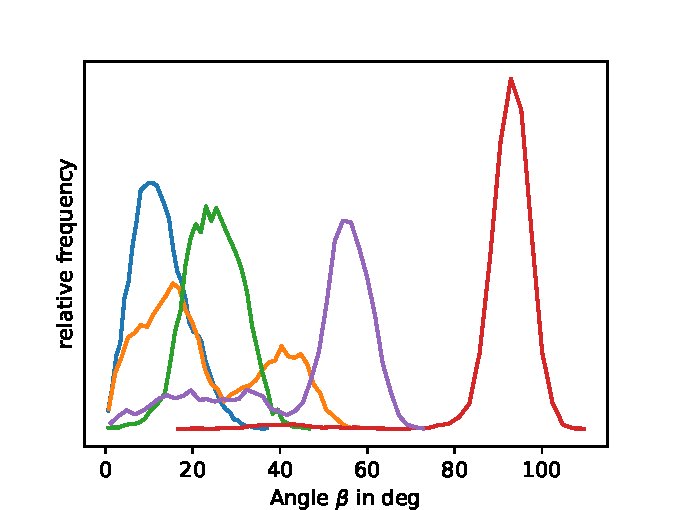
\includegraphics[height=5cm]{figures/introduction/sara_angles}
	}\hfill%
	\subcaptionbox{\label{stabil:forceillustr}}[0.49\textwidth]{
		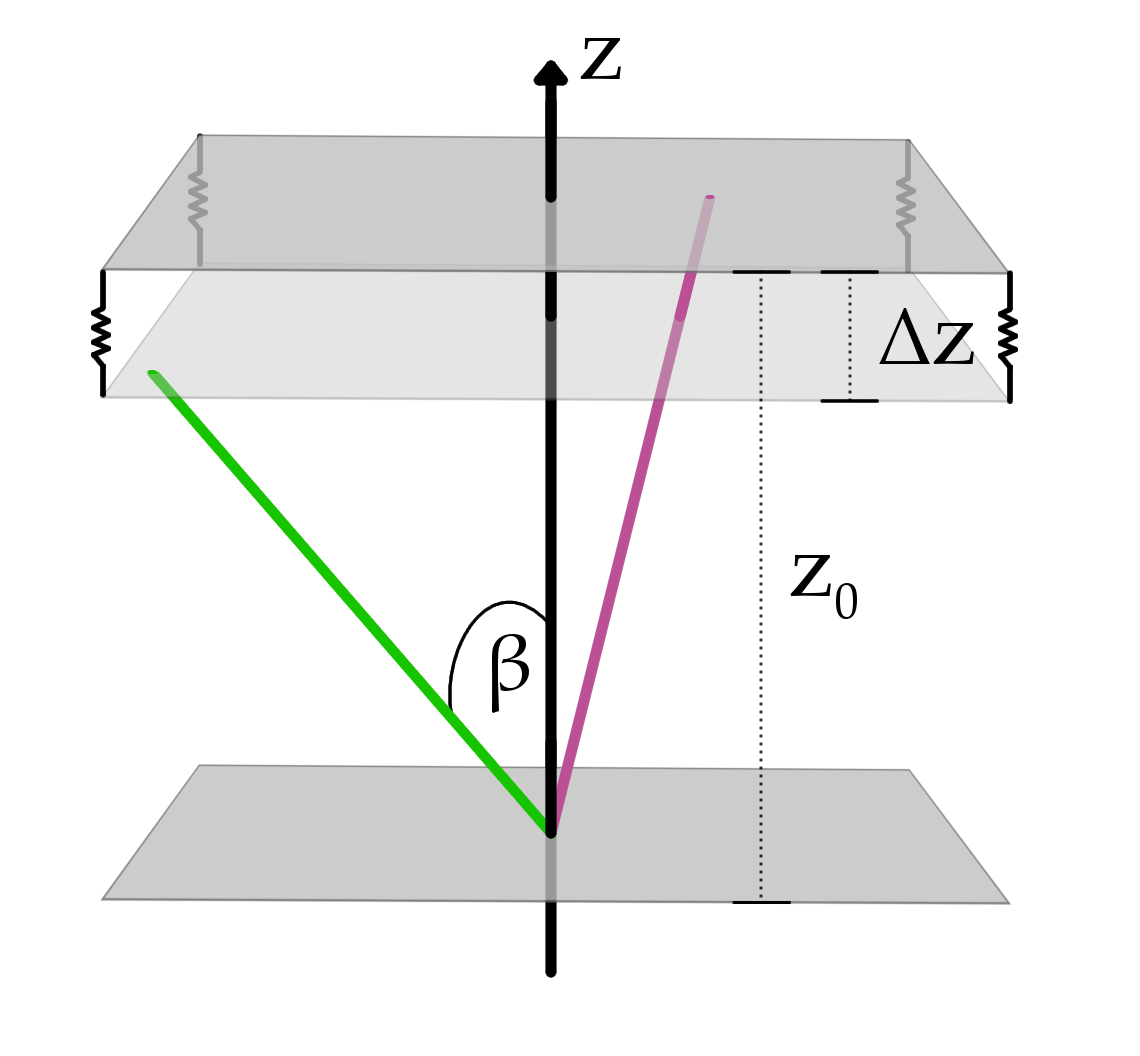
\includegraphics[height=5cm]{figures/introduction/forceapproach}
	}%
	\nicecaption{Stabilising force}{(\subref{stabil:sarascurves}): Distributions of $\beta$ obtained by \textcite{sara}. The red curve shows the distribution for a fallen FAK. The blue and green curve are consistent with equivalent all-atom simulations in \charmm{}.  (\subref{stabil:forceillustr}): Illustration of the stabilising force. The violet line represents a orientation of $\vec{d}_{F}$ which wouldn't lead to a force ($\Delta z = 0$). The green line represents a orientation which leads to an uplift ($\Delta z > 0$, the springs are tensioned). The force is proportional to $\Delta z$.}
\end{figure}
%
%
%
\section{Setup 3 - FAK on \pip{}-containing membrane}
\label{setup:setup3}
Setup 3 is a \martini{} simulation adopted from \textcite{sara}. It contains a single FAK molecule which was placed on a phosphatidylcholine (\popc{}) and \pip{} membrane (\pip{} concentration $15\%$). NaCl ions were added to neutralize the system (see \autoref{setup:setup3_pic}). In contrast to \textcite{sara}, we applied the stabilizing force explained in \autoref{motivation} to the protein.\\
Five independent copies were simulated for $10\,\si{\micro\second}$ each. The temperature was kept at $300\si{\kelvin}$ and the default parameters of \martini{} were used.
%
%
%
\begin{figure}[h]
	\centering
	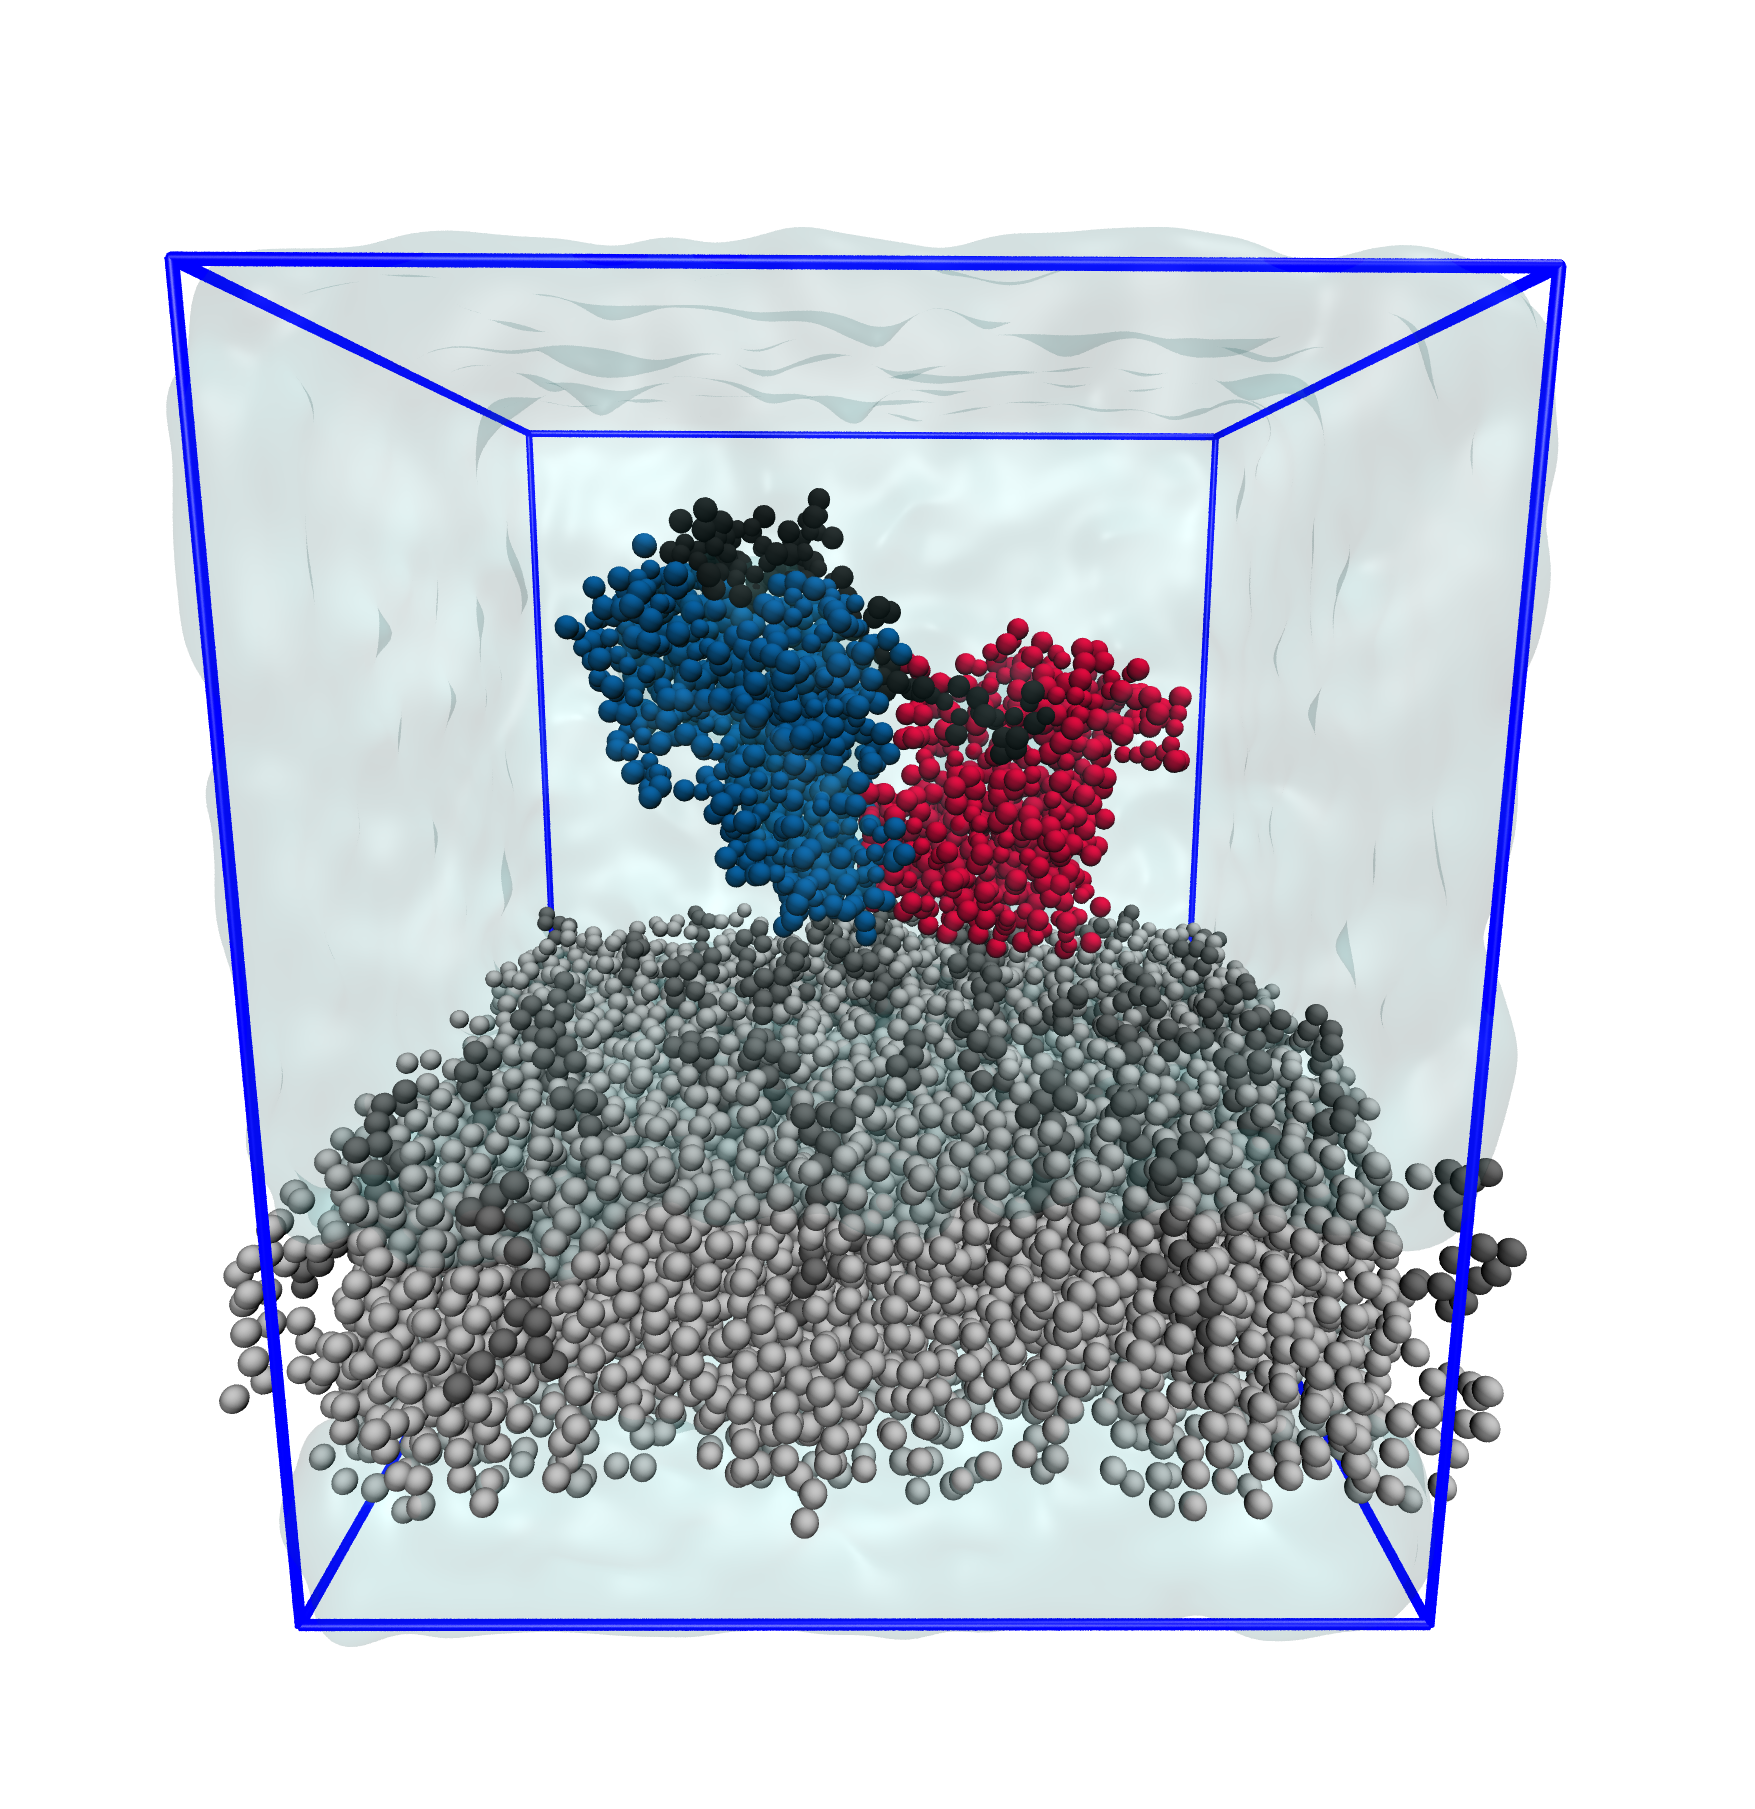
\includegraphics[height=6cm]{figures/setup/setup_gen}
	\nicecaption{Setup 3 - FAK on a \pip{} membrane}{The setup involves one FAK molecule (FERM blue, kinase red and linker black, 1486 beads) on top of a \pip{} containing membrane (667 \pope{} lipids, 54 \pip{} lipids, ca. 22000 membrane beads in total). The surrounding solution consists of ca. 21400 solvent beads and 473 ions. The box dimensions are $15.2\,\si{\nano\metre}$ x $15.2\,\si{\nano\metre}$ x $17.0\,\si{\nano\metre}$.}
	\label{setup:setup3_pic}
\end{figure}
%
%
%
\section{Setup 4 - FAK cluster}
From each copy in setup 3, we cut out five frames. All these 25 frames were arranged on a {5x5} grid (\autoref{setup:setup4_pic}). Each of the 25 proteins was stabilized with the external force independently. After a short equilibration the system was simulated for $9\,\si{\micro\second}$. We set up 25 different copies (regarding the arrangement of the frames) which resulted in a total simulation time of $45\,\si{\micro\second}$. The temperature was kept at $300\,\si{\kelvin}$ and the default parameters of \martini{} were used.
%
%
%
\begin{figure}[h]
	\centering
	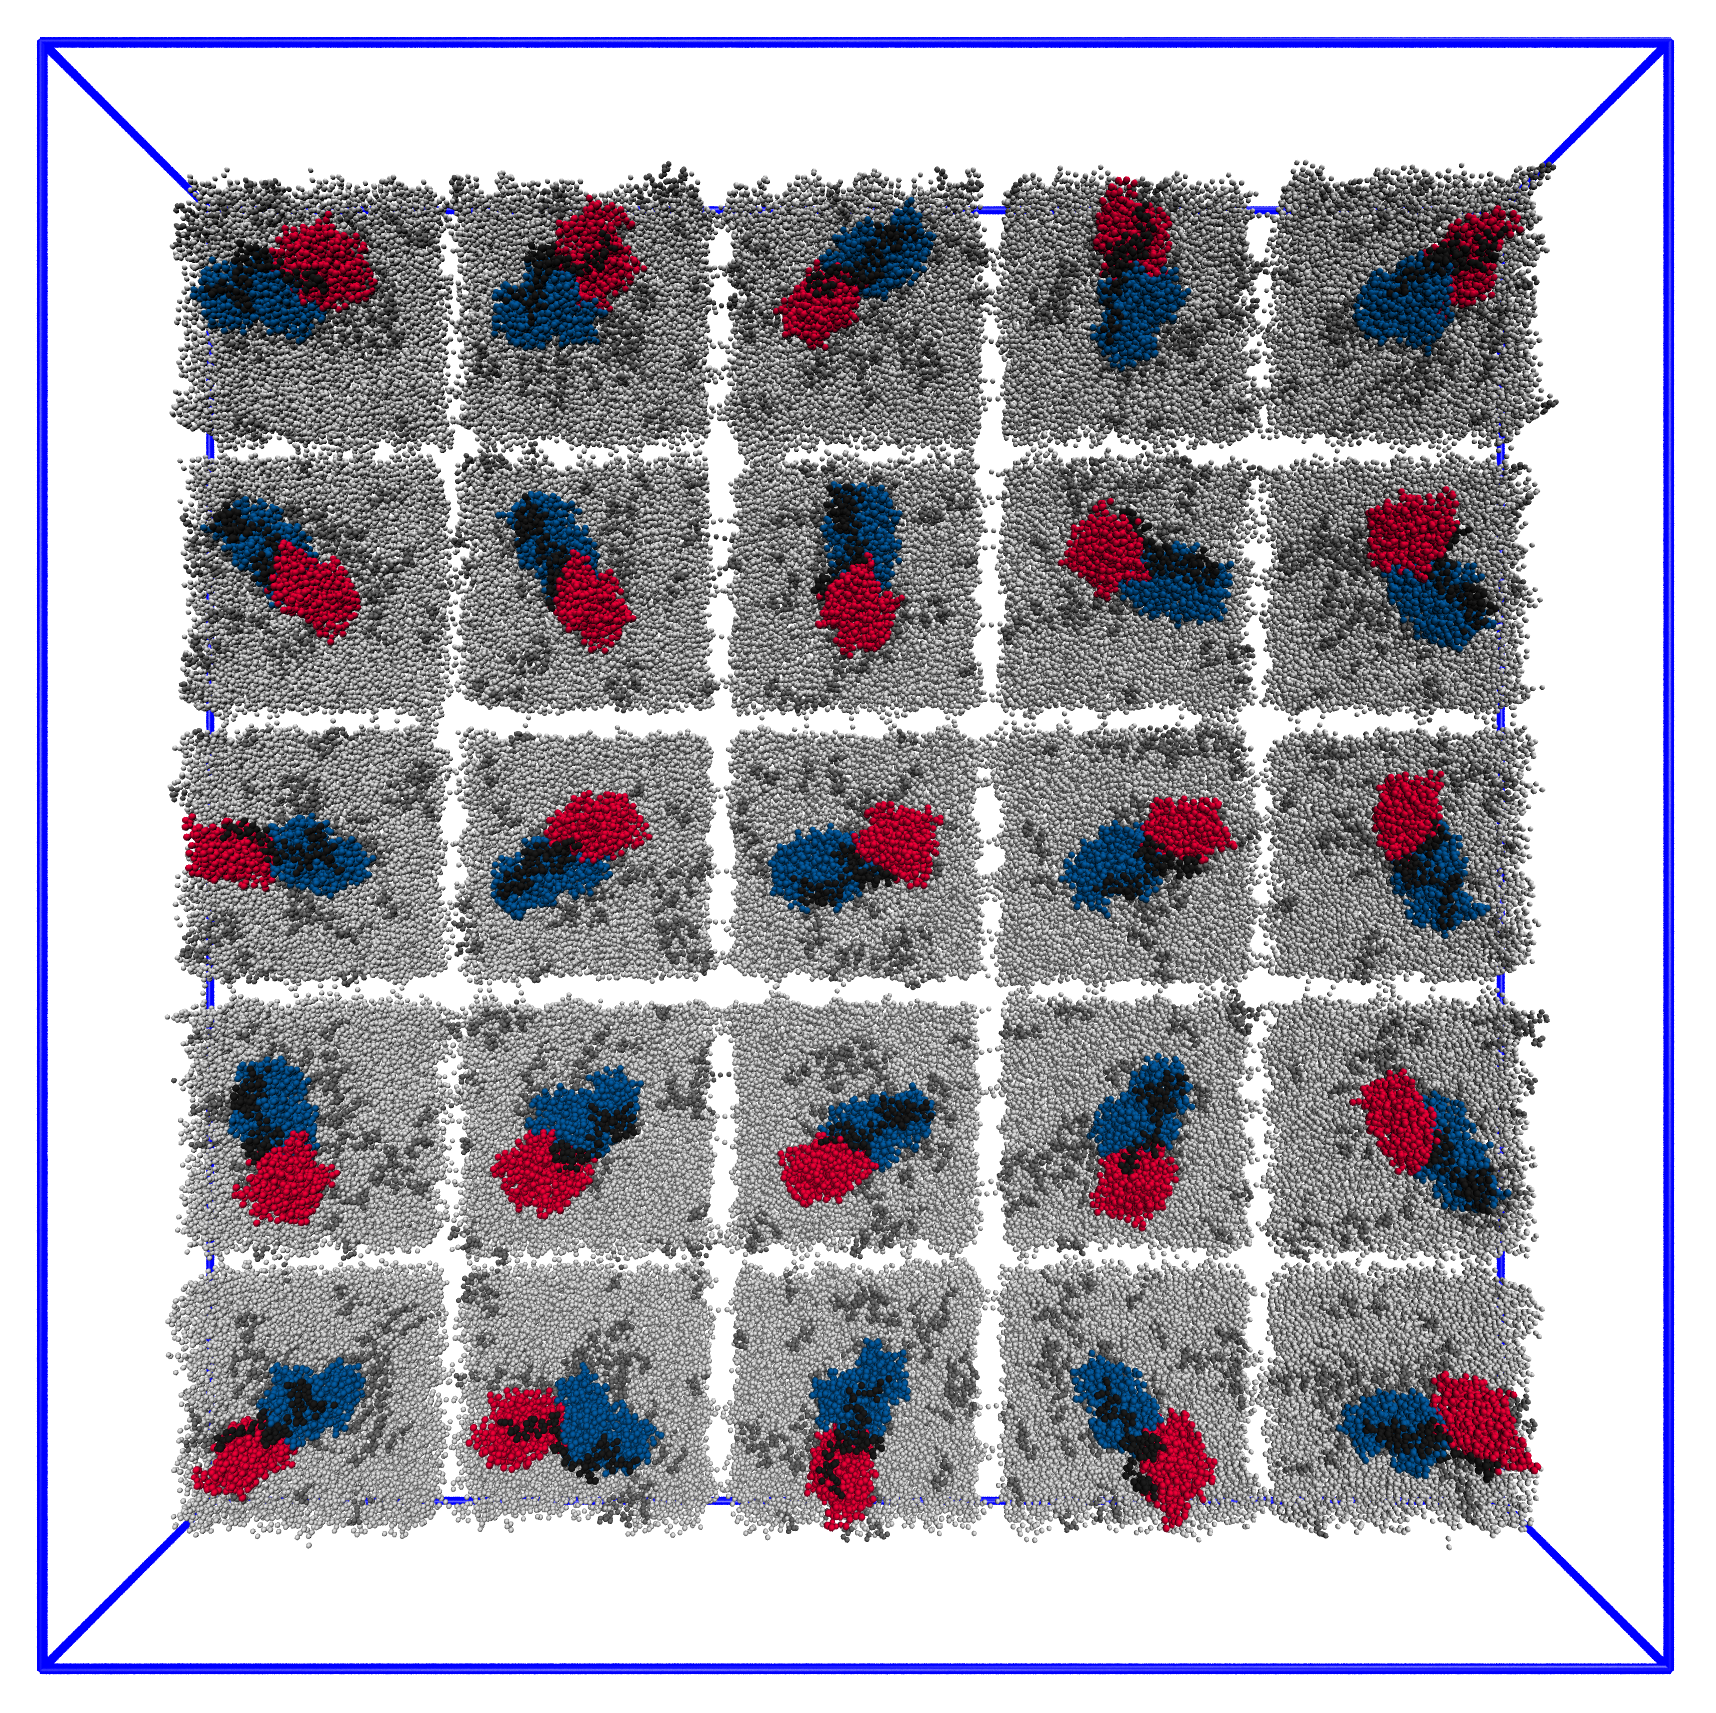
\includegraphics[height=6cm]{figures/setup/setup_cluster}
	\nicecaption{Setup 4 - FAK cluster}{The setup is a combination of 25 frames from \autoref{setup:setup3}. It consists of ca. 807000 beads in a box of size $80.0\,\si{\nano\metre}$ x $80.0\,\si{\nano\metre}$ x $17.0\,\si{\nano\metre}$. The spaces between the frames were needed during setup to avoid an overlapping of the beads, but disappears during the equilibration.}
	\label{setup:setup4_pic}
\end{figure}
%
%
%